\documentclass[12pt,a4paper]{report}

\usepackage[margin=2.5cm]{geometry}
\usepackage{graphicx}
\usepackage{booktabs}
\usepackage{caption}
\usepackage{subcaption}
\usepackage{siunitx}
\usepackage{amsmath}
\usepackage{tikz}
\usepackage{pgfplots}
\usepackage{hyperref}
\usepackage{enumitem}
\usepackage{longtable}
\usepackage{multirow}
\usepackage{titlesec}
\usepackage{fancyhdr}
\usepackage{setspace}
\usepackage[backend=biber,style=numeric]{biblatex}
\usepackage{pdfpages}

\hypersetup{
    colorlinks,
    linkcolor={red!50!black},
    citecolor={blue!50!black},
    urlcolor={blue!80!black}
}

\addbibresource{Thermal.bib}
\setstretch{1.2}

\pgfplotsset{compat=1.18}

\title{Electric Conversion of Assist Vehicle}
\author{Brian McKenna -- Launceston \& North East Railway}
\date{\today}

\begin{document}
\maketitle
\tableofcontents
\newpage

\chapter{Project overview}

\section{Introduction}

This document provides a detailed engineering risk assessment and mitigation plan for thermal runaway in the modified assist vehicle operated by the Launceston \& North East Railway (L\&NER). The original Briggs \& Stratton petrol engine has been replaced with a QS165 electric traction motor powered by an 18S3P lithium-ion battery pack using LG E63B NCM cells and controlled by a JK Smart Battery Management System (BMS).

The purpose of this report is to demonstrate that the electrical conversion and associated energy storage system are designed, installed, and managed to eliminate or minimise, so far as is reasonably practicable, the risks of fire, explosion, or injury associated with thermal runaway.

This report has been prepared by Brian McKenna, the primary engineer on this electric conversion project. He is a software engineer who has worked in the renewable energy industry and has implemented software for Battery Management Systems.

\section{Rationale for Electric Conversion}

The decision to replace the original 13.5~HP Briggs \& Stratton petrol engine with an electric traction system was made to improve environmental performance, operational reliability, and safety, while aligning with the Launceston \& North East Railway’s broader sustainability objectives. The original internal combustion engine produced significant exhaust noise and emissions that detracted from the natural ambience of the Tasmanian bushland and it would reduce the comfort of visitors on adjacent pedal-powered rail vehicles. 

Electrification eliminates exhaust emissions entirely, contributing to improved air quality and a quieter, more enjoyable experience for tourists and volunteers. Electric drive systems operate almost silently apart from drivetrain noise, allowing the natural soundscape of the railway corridor to be preserved.

From a maintenance perspective, the electric traction system greatly reduces mechanical complexity. The previous petrol engine required regular servicing, including oil changes, fuel system maintenance, and exhaust management. The new QS165 motor and FarDriver controller have minimal moving parts, resulting in reduced wear, simpler fault diagnosis, and lower lifetime maintenance costs.

Operational control and safety are also enhanced. An electric system provides instant torque without the risk of stalling, and electric motor controllers enforce programmable current and speed limits, reducing the potential for operator error. The battery management and isolation systems ensure that electrical faults or overtemperature conditions are automatically detected and managed, further improving reliability and safety.

The conversion supports the railway’s long-term vision for low-impact, sustainable transport. By demonstrating successful electrification of a small traction vehicle, the project establishes a scalable model for future conversions and contributes to the organisation’s technical capability in electric mobility. It also demonstrates leadership in environmental stewardship -- minimising disturbance to wildlife, reducing fire risk associated with fuel handling, and aligning with community expectations for modern, sustainable tourism operations.

\section{System Requirements}

The electric conversion of the former petrol-powered maintenance vehicle was guided by a defined set of functional, performance, and safety requirements, ensuring that the resulting traction system is reliable, efficient, and suitable for mixed-use operation on the heritage railway. These requirements reflect operational needs, environmental conditions, and applicable safety principles relevant to the Launceston \& North East Railway.

\subsection{Functional Requirements}
\begin{itemize}
    \item The vehicle must provide sufficient tractive effort to haul three loaded railbug vehicles (each carrying two adults and two children) uphill on the steepest section of track, which has a gradient of 1:40.
    \item Regenerative braking or controlled deceleration must be supported to ensure smooth operation on downhill gradients.
    \item The system must allow simple forward and reverse operation with minimal operator training.
    \item The vehicle must be capable of operating for at least 2~hours under mixed-load conditions without recharge.
\end{itemize}

\subsection{Performance Requirements}
\begin{itemize}
    \item The drive system must deliver sufficient wheel torque to overcome both rolling resistance and the gravitational load associated with a 1:40 gradient.
    \item The system should achieve a maximum service speed of 15~km/h on level track.
    \item Acceleration should be smooth and controllable, avoiding wheel slip or jerking motion.
\end{itemize}

\subsection{Safety and Reliability Requirements}
\begin{itemize}
    \item All electrical systems must comply with the relevant provisions of \textbf{AS/NZS~5139:2019}, including protection against short circuit, overcurrent, insulation failure, and thermal hazards.
    \item The traction battery must incorporate BMS-controlled protection and isolation, with appropriate fusing and contactors to safely disconnect in the event of a fault.
    \item The motor controller must provide programmable current, voltage, and temperature limits to prevent component damage and unsafe operating conditions.
    \item Mechanical systems (mounts, couplings, and axles) must be designed and installed by qualified personnel to withstand operational loads with suitable safety margins.
    \item The system must include an emergency isolation switch accessible to the operator and external responders.
\end{itemize}

\subsection{Environmental and Operational Requirements}
\begin{itemize}
    \item The conversion must reduce noise and emissions, improving the visitor experience and reducing disturbance to wildlife.
    \item The system must be suitable for outdoor use in the Tasmanian environment, including operation in light rain, variable temperatures, and exposure to dust and vegetation.
    \item Maintenance requirements must be reduced relative to the petrol engine, with minimal need for fluid changes or mechanical adjustments.
\end{itemize}

\section{Traction Motor Requirements and Torque Analysis}

The electric traction system must provide sufficient torque and power to safely and reliably propel a consist of up to three railbug vehicles along the Launceston \& North East Railway’s 3.3~km demonstration track. This includes operation on the steepest gradient section of approximately 1:40, while carrying typical passenger loads and maintaining controlled performance during start-up, acceleration, and regenerative braking.

\subsection{Operational Scenario}

Each railbug vehicle is designed to carry approximately two adults and two children, with a total loaded mass (including the vehicle structure) estimated at 400~kg per unit. When operating as a three-vehicle consist, the combined rolling mass including the powered vehicle and driver is estimated at approximately 1,400~kg.  

The traction system must therefore be capable of initiating motion from rest, sustaining steady-state operation at the desired cruise speed, and providing sufficient tractive effort to overcome both rolling resistance and gravitational load on the 1:40 incline.

\subsection{Gradient and Rolling Resistance}

The total tractive force required can be approximated as the sum of rolling resistance and the component of weight acting along the incline:

\[
F_\text{total} = F_\text{roll} + F_\text{grade}
\]

Rolling resistance is taken as approximately \(0.0025\,W\) for steel wheel on steel rail conditions, where \(W\) is the vehicle weight. The grade resistance on a 1:40 slope is given by:

\[
F_\text{grade} = \frac{W}{40}
\]

For the estimated consist weight of 1,400~kg (13,734~N), this yields:

\[
F_\text{roll} = 0.0025 \times 13{,}734 = 34.3~\text{N}
\]
\[
F_\text{grade} = \frac{13{,}734}{40} = 343~\text{N}
\]
\[
F_\text{total} = 34.3 + 343 = 377~\text{N}
\]

\subsection{Torque Requirement at the Wheels}

Assuming a wheel radius of 0.6~m, the torque at the wheels required to overcome this tractive load is:

\[
T_\text{wheel} = F_\text{total} \times r = 377 \times 0.6 = 226~\text{N·m}
\]

This represents the steady-state torque demand for climbing the maximum gradient at constant speed. To allow for acceleration, minor gradients, bearing friction, and inefficiencies, a design safety margin of at least 2–3 times this value is recommended, yielding a peak requirement in the order of 450–700~N·m at the wheels.

\subsection{Power Requirement}

The required power depends on the desired operating speed. For example, at a steady climb of 10~km/h (2.78~m/s):

\[
P = F_\text{total} \times v = 377 \times 2.78 = 1.05~\text{kW}
\]

This is the theoretical minimum continuous power. Considering transmission losses, acceleration, and variable gradients, a continuous rating of approximately 3–4~kW and a short-term peak capability of 8–10~kW are appropriate design targets for the traction system

\subsection{Design Implications}

The chosen traction motor, gearing, and drive system must therefore satisfy the following criteria:

\begin{itemize}
  \item Provide at least 700~N·m of peak torque at the wheels to ensure safe starting and hill-climbing.
  \item Sustain approximately 200–250~N·m of continuous torque for steady operation on inclines.
  \item Deliver a continuous power output of at least 3~kW.
  \item Allow regenerative braking capability for controlled descent and energy recovery.
\end{itemize}

These requirements form the performance baseline for evaluating and selecting a suitable motor and controller combination for the converted vehicle.

\section{Component Selection and Integration}

The component selection for the electric conversion was guided by principles of safety, availability, cost efficiency, and technical compatibility with the existing vehicle structure and battery system. The design aimed to maximise the use of proven, mass-produced electric vehicle components, while repurposing available assets to minimise waste and cost.

\subsection{Design Verification}

Brian McKenna developed a software physics simulation of the vehicle to verify the requirements and potential solution. The simulation software is documented in Appendix \ref{ch:simulation}. By allowing quick experimentation of masses, gradient, rolling resistance, motor power, gearing, and target speed, the simulation gives an immediate sense of whether a given configuration is physically feasible and how close it is to its limits.

The simulation tool revealed that the components should be powerful enough, but not by a large margin. The gear ratio played a major factor and the simulation showed that changing the gearing could increase the margin by a lot, if needed. The simulation gave Brian McKenna and Greg Stewart sufficient confidence in the requirements and the design that the project proceeded.

\subsection{Battery System}

The battery system is composed of repurposed Hyundai Kona~EV lithium-ion modules that were previously used in the organisation’s off-grid energy storage system. These modules were selected for their high energy density, well-documented performance, and integrated safety design compliant with \textbf{AS~IEC~62619:2022}. Their reuse in this application reduces environmental impact and ensures consistency with existing maintenance and monitoring experience within the organisation. 

The battery pack arrangement is described with detail in \ref{sec:pack-configuration}. Battery management and protection are provided by a JK-BMS unit, chosen for its programmable protection thresholds, integrated cell balancing, and communication capability.

\subsection{Traction Motor and Controller}

A QS165 brushless permanent magnet motor was selected to provide tractive power. This model is widely used in electric motorcycles and light utility vehicles, offering a favourable balance of torque, efficiency, and cost. The motor’s compact form factor, sealed construction, and rated torque output make it well suited to low-speed rail operation and outdoor conditions typical of the Launceston \& North East Railway.

Motor control is provided by a FarDriver~72450 controller, which is widely supported and specifically matched to the QS165 motor family. The controller provides comprehensive programmability of current limits, torque curves, regenerative braking, and thermal protection. Its use of standard CAN and UART interfaces allows for future data logging and integration with onboard monitoring systems. Both the motor and controller combination are rated for substantially higher power levels than required in this application, ensuring ample thermal and electrical headroom.

\subsection{Mechanical Integration}

The mechanical integration of the motor and drivetrain was overseen and executed by Greg Stewart, a qualified Motor Mechanic (Lic No: 7277 10508 025470) with extensive experience in vehicle fabrication. His mechanical review involved a comprehensive overhaul of the chassis, which was deemed necessary after the original vehicle was found to be in an unsafe condition, featuring misaligned wheels, a failing petrol motor mount and crooked transmission. The mounting brackets, axle supports, and sprocket assemblies were fabricated to suit the new configuration, ensuring proper alignment, chain tension, and structural integrity under load.

\subsection{Rationale and Compatibility}

The use of mass-produced components such as the QS165 motor and FarDriver controller ensures that replacement parts, configuration tools, and technical documentation are readily available. These components have been adopted by a large community of electric vehicle builders, providing confidence in their reliability and long-term support. By repurposing Hyundai Kona EV modules and employing an accessible BMS system, the project achieves a high standard of safety and functionality without the cost or complexity of a bespoke commercial drive package.

The resulting system provides a compact, efficient, and quiet electric drivetrain that aligns with the railway’s commitment to sustainable operation and minimal environmental impact.

\section{Traction Motor Replacement and Controller Integration}

\subsection{Scope of Modification}
The original 13.5~HP Briggs \& Stratton internal combustion engine has been replaced
with a QS165 brushless DC motor controlled by a FarDriver 72450 motor controller. This
modification includes mechanical integration of the motor to the vehicle chassis, installation
of new axles and sprockets, and connection to the existing battery system. All structural
components affected by the modification have been designed and fabricated to withstand
dynamic and static loads encountered during normal operation along the 3.3~km track.

\subsection{Technical Description}
The QS165 motor delivers continuous and peak torque suitable to meet or exceed the
performance of the original engine. The FarDriver 72450 controller provides programmable
current limits, motor speed control, and overtemperature protection. Mechanical integration
was carried out by a qualified mechanic, ensuring precise alignment of the motor shaft with
the sprocket and axle assemblies to prevent undue wear or vibration. All drive components
have been designed with safety factors appropriate to expected operational stresses.

During the technical review of the original propulsion system, it was discovered that the rear differential top pulley and input shaft bearing had failed, with evidence of unsafe past repairs, including a pulley welded out of square. Consequently, the decision was made to strip the vehicle to its chassis and implement a completely rebuilt rear end. The modification included strengthening and reinforcing the rear chassis, removing the obsolete differential entirely, and installing a new rear axle with a motorcycle-grade chain and sprocket drive system.

\subsection{Risk Assessment and Mitigation}
Primary risks unique to the motor replacement include:
\begin{itemize}
  \item Mechanical failure of drive components (motor couplings, sprockets, axles).
  \item Excessive torque or unintended motion due to controller or operator error.
  \item Motor or controller overtemperature during high load conditions.
\end{itemize}

Mitigations specific to these risks include:
\begin{itemize}
  \item Secure mechanical mounting with robust fabrication and alignment verification.
  \item Integration of the motor controller with an emergency isolation switch.
  \item Bench and on-track commissioning under controlled conditions to verify
        motor performance, alignment, and thermal behavior.
  \item Operator training on safe start-up, operation, and emergency procedures
        unique to the traction system.
\end{itemize}

\subsection{Operational Procedures and Commissioning}
Pre-start inspections focus on mechanical integrity (mounts, couplings, and drive components)
and controller functionality. The motor controller enforces current and speed limits to
prevent over-torque conditions. On-track commissioning involved a controlled round-trip
on the 3.3~km track, monitoring motor performance, vibration, and mechanical alignment.
Results are recorded for baseline reference and future comparison. Scheduled post-implementation
reviews are conducted after initial operating hours and annually thereafter to ensure ongoing
mechanical and operational safety.

\subsection{Braking System Independence and Adequacy}
The vehicle utilizes a standard e-bike braking architecture that provides dual-layered deceleration through integrated physical and electronic controls. The primary stopping power is delivered by the original physical disc brakes, which have been retained without modification to ensure that the fundamental braking performance remains consistent with the vehicle’s original design. These mechanical brakes are supplemented by the FarDriver 72450 controller, which is programmed to provide regenerative braking for controlled descents and energy recovery.

A critical feature of this configuration is that the physical disc braking system operates entirely independently of the electric drive-train, including the motor, controller, and chain drive. This independence guarantees that effective, fail-safe mechanical braking is always available to the operator, even if the drive-train fails or the electrical system is isolated.

Furthermore, the braking system is considered highly adequate despite the removal of the original petrol motor’s transmission braking. Because the maximum service speed is strictly limited to 15 km/h, the original disc brakes possess more than enough capacity to safely stop the vehicle under all expected operational loads. The supplemental regenerative braking further reduces wear on the physical components while providing a smooth, controlled deceleration profile.

\subsection{Mechanical Engineering Review}

A mechanical review of the vehicle's modifications was conducted by Greg Stewart, a qualified Motor Mechanic (Lic No: 7277 10508 025470) and long-standing board member of the Launceston \& North East Railway. His initial assessment of the vehicle in its original petrol-powered configuration identified several critical safety defects, including significant wheel misalignment, a failing motor mount and non-functional brakes. Further inspection revealed a total failure of the rear differential input shaft bearing and a drive pulley that had been dangerously welded out of square, a condition deemed likely to cause catastrophic failure during operation.

Given the obsolescence of the original transmission components, the vehicle was stripped to its chassis and subjected to a complete engineering overhaul. The rear chassis was strengthened and reinforced to accommodate a new rear axle and a motorcycle-grade chain and sprocket drive system. This assembly includes a custom-fabricated steel engine mount and an integrated automatic chain tensioner, designed specifically to manage the increased torque and power profile of the QS165 electric motor.

The review also verified the implementation of a redundant braking architecture consisting of the original manual disc brakes and supplemental regenerative braking via the motor controller. Through these modifications, the unit has been transformed into a mechanically robust vehicle that tracks precisely without derailing, representing a significant improvement in safety and reliability over the original configuration. Comprehensive photographic evidence has been maintained throughout the build process (\ref{subsec:timeline}) to provide a transparent record of all engineering improvements and mechanical verifications.

\section{Dashboard}

During development of the vehicle, it became apparent that a clear indication was needed when the motor controller is powered and the vehicle is able to move. A prominent amber beacon light was installed on the dashboard. This light provides an immediate visual confirmation that the ignition is on and the vehicle is live, compensating for the absence of the usual audible cues associated with an engine.

A large red emergency stop button was chosen as the start/stop mechanism. The operator must twist the button to start the vehicle and it's very quick and obvious to stop the vehicle, which is critical in an emergency. This button is the primary mitigation against electrification risks, and can be pressed to immediately cut power if there's any indication of smoke, a burning smell or exposed wiring. The button cuts power to the controller, immediately stopping any unintended motion or controller errors.

A digital speedometer was added so that the operator can accurately regulate the vehicle. The speedometer uses GPS and it is quite accurate and independent of the motor controller. The speedometer has an upper limit of 30 km/h which is more than adequate for our needs but still gives a good amount of fidelity.

A battery level indicator measures and shows the battery's voltage and provides a visual representation of State of Charge using bars, just like many mobile phones or other battery devices. The meter is not accurate under load, since it doesn't do coulomb counting, but it is sufficient enough to provide a useful indication of whether the vehicle needs to be charged or is "full" at our designated 80\% maximum.

The existing horn was retained in order to be able to alert others to the vehicle's presence, which has become more important now that the vehicle itself does not emit much noise.

The FarDriver controller is highly configurable through software. Brian McKenna used this software to create an initial controller profile. Maximum RPM, torque curves, regenerative braking and voltage limits were all changed to values appropriate to the vehicle's requirements.

An electrical schematic diagram and parts list of the above components is available in Appendix \ref{ch:schematic}.

A standard class A fire extinguisher was mounted to the vehicle in case of fire. Special Lithium-ion fire extinguishers are available, but they are very expensive and are not able to effectively stop or control thermal runaway \cite{en13195117}. This fire extinguisher should primarily be used to prevent the spread of a fire, keeping it away from the battery.

The Safey Management System documents which referenced parts of the escort vehicle been updated and attached in Appendix \ref{ch:sms}.

\chapter{Project implementation}

\section{Timeline}

\label{subsec:timeline}

\begin{longtable}{p{3.5cm} | p{9.5cm}}
\textbf{Date} & \textbf{Work} \\ \hline
1 September 2024 & L\&NER decided to convert the petrol propulsion \ref{fig:before} to electric. \\
17 October 2024 & Greg Stewart and Brian McKenna investigated options for mounting the motor \ref{fig:motorplacement} \ref{fig:motorshaft}. \\
23 October 2024 & Greg Stewart finished fabrication of a motor mount \ref{fig:motormount1} \ref{fig:motormount2}. \\
29 October 2024 & Pulley arrived. After Greg Stewart attempt at fitting, he determined that the pulley was too large \ref{fig:pulley1}. \\
19 November 2024 & A smaller pulley was machined to fit the vehicle \ref{fig:pulley2}. \\
23 November 2024 & While fitting the smaller pulley, Greg Stewart discovered that the transmission pulley was wobbling, makiing it unsafe for operation \ref{fig:transmission}. \\
4 December 2024 & After not being able to find a replacement transmission, Greg Stewart and Brian McKenna decided to move to a chain drive, removing the transmission altogether \ref{fig:motorsprocket} \ref{fig:axlesprocket}. \\
20 December 2024 & Greg Stewart finished fabrication of motor and controller mounts \ref{fig:controllermount} \ref{fig:motormount3}. Ian Nicholas finished fabrication of sprocket-axle coupling \ref{fig:axlecoupler}. \\
31 December 2024 & Greg Stewart mounted the motor, controller and axle to the vehicle \ref{fig:chassismounted}. \\
11 January 2025 & Brian McKenna lifted the vehicle and tested the batteries, motor and controller. \\
13 January 2025 & Greg Stewart fabricated an automatic chain tensioner \ref{fig:tensioner}. \\
3 February 2025 & Greg Stewart fabricated a battery rack \ref{fig:batteryrack}. Brian McKenna added branding stickers. \\
8 February 2025 & Greg Stewart and Brian McKenna did a test on the rail at Turners Marsh station \ref{fig:testride}. \\
15 March 2025 & Brian McKenna fitted a fuse \ref{fig:fuse}, beacon light, emergency stop \ref{fig:initialdash} and charger \ref{fig:charger}. \\
18 March 2025 & Brian McKenna created a wiring loom for the Battery Management System (BMS) \ref{fig:bmsloom}. \\
21 March 2025 & Greg Stewart and Brian McKenna put the batteries and BMS into the vehicle \ref{fig:batteryandbms}. \\
30 March 2025 & Brian McKenna configured the BMS \ref{fig:screenshotbms} and Fardriver controller \ref{fig:screenshotfardriver}. \\
11 July 2025 & Ian Nicholas modified the axle-sprocket coupling and Greg Stewart attached a larger sprocket \ref{fig:axlesprocket2}. \\
5 December 2025 & Brian McKenna and Greg Stewart installed the completed dashboard \ref{fig:dashboard}.
\end{longtable}

\chapter{Battery safety}

\section{Battery System Description}

\subsection{Pack Configuration}
\label{sec:pack-configuration}

The battery modules have been sourced from a wrecked Hyundai Kona EV. Each module has the following specifications \cite{LG_E63B_datasheet}:

\begin{itemize}
  \item \textbf{Cell type:} LG E63B (NCM chemistry)
  \item \textbf{Configuration:} 9S3P
  \item \textbf{Nominal voltage:} \(9 \times 3.65 = 32.9\,\mathrm{V}\)
  \item \textbf{Nominal capacity:} \(3 \times 63\,\mathrm{Ah} = 189\,\mathrm{Ah}\)
  \item \textbf{Total energy:} \(32.9\,\mathrm{V} \times 189\,\mathrm{Ah} \approx 6.2\,\mathrm{kWh}\)
  \item \textbf{Enclosure:} Aluminium frame with temperature monitoring
\end{itemize}

We chose to use two of these modules for the conversion because they were readily available and would fit perfectly under the vehicle's existing hood, while giving a useful voltage for existing traction motor components. In total, this gave us an 18S3P pack with 12.4kWh rated capacity.

\subsection{BMS Overview}

In order to make the project modular, easy to repair and affordable, we decided to go with a popular JK BMS product. L\&NER already had some familiarity with these products after using them our off-grid storage shed.

The JK-BD6A24S12P provides:

\begin{itemize}
  \item Per-cell voltage monitoring and active balancing of 0.6A
  \item Temperature sensing
  \item Overvoltage/undervoltage cutoff
  \item Overcurrent protection
  \item Charge/discharge MOSFET isolation
  \item Communication (Bluetooth/RS485)
\end{itemize}

\section{Understanding Thermal Runaway in NCM Cells}

\subsection{Definition and Mechanism}

Thermal runaway is a self-sustaining exothermic reaction within a lithium-ion cell caused by internal short-circuit, overcharging, or external heating. It involves three main stages:

\begin{enumerate}
  \item \textbf{SEI layer breakdown} (\(\sim90{-}120\,^{\circ}\mathrm{C}\)): destabilises the anode, releasing heat and gases.
  \item \textbf{Electrolyte decomposition} (\(130{-}170\,^{\circ}\mathrm{C}\)): produces additional heat and flammable vapours.
  \item \textbf{Cathode oxygen release} (\(180{-}220\,^{\circ}\mathrm{C}\)): NCM cathodes release oxygen, fueling combustion.
\end{enumerate}

\subsection{Propagation Risk}

If the heat from one cell is not adequately dissipated, neighbouring cells can reach decomposition temperature, leading to propagation. This risk is strongly influenced by:
\begin{itemize}
  \item State of charge (SOC)
  \item Cell spacing and enclosure design
  \item Presence of flammable vapour and ignition sources
\end{itemize}

\section{Operating Regime and Voltage Limitation}

Figure~\ref{fig:soc-curve} shows the open-circuit voltage (OCV) versus SOC for the LG E63B cells. L\&NER limits charge to 4.0\,V per cell, corresponding to approximately 85\% SOC.

\begin{figure}[h!]
  \centering
  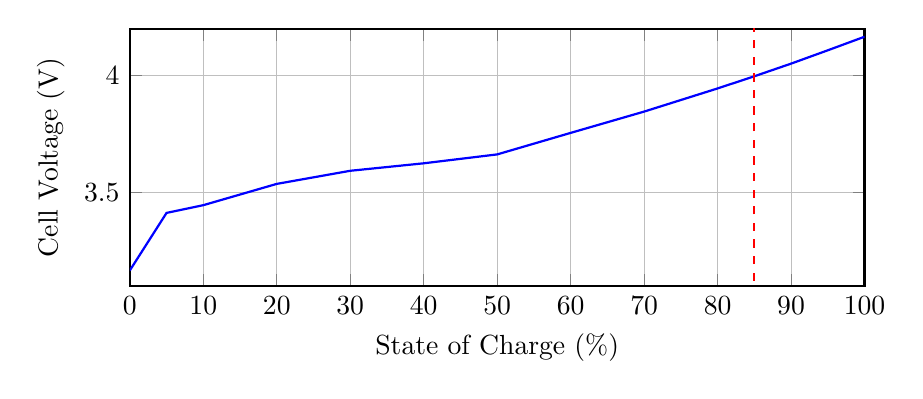
\begin{tikzpicture}
    \begin{axis}[
      width=0.9\textwidth,
      height=0.4\textwidth,
      xlabel={State of Charge (\%)},
      ylabel={Cell Voltage (V)},
      grid=both,
      xmin=0, xmax=100,
      ymin=3.1, ymax=4.2,
      thick
    ]
      \addplot+[mark=none] coordinates {
        (0,3.167) (5,3.413) (10,3.446) (20,3.537) (30,3.593)
        (40,3.625) (50,3.663) (60,3.755) (70,3.846) (80,3.945)
        (85,3.997) (90,4.051) (95,4.108) (100,4.166)
      };
      \addplot [red, dashed, thick] coordinates {(85,0) (85,5)};
    \end{axis}
  \end{tikzpicture}
  \caption{OCV vs SOC for LG E63B cells. The 4.0\,V limit corresponds to 85\% SOC, significantly reducing chemical instability risk.}
  \label{fig:soc-curve}
\end{figure}

\begin{figure}[h!]
\centering
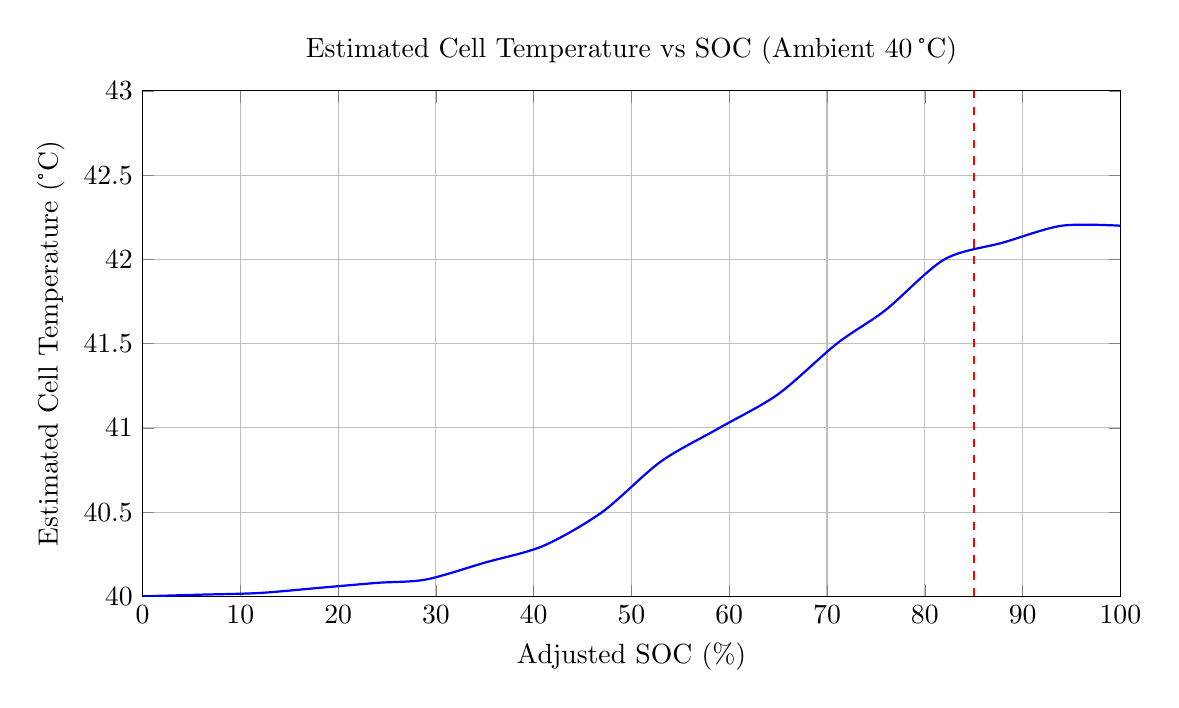
\begin{tikzpicture}
\begin{axis}[
    width=14cm, height=8cm,
    xlabel={Adjusted SOC (\%)},
    ylabel={Estimated Cell Temperature (°C)},
    grid=both,
    ymin=40, ymax=43,
    xmin=0, xmax=100,
    title={Estimated Cell Temperature vs SOC (Ambient 40\,°C)},
]

% Temperature rise estimates (ΔT added to 40°C ambient)
\addplot[smooth, thick, blue] coordinates {
    (0,40.0)
    (6,40.01)
    (12,40.02)
    (18,40.05)
    (24,40.08)
    (29,40.1)
    (35,40.2)
    (41,40.3)
    (47,40.5)
    (53,40.8)
    (59,41.0)
    (65,41.2)
    (71,41.5)
    (76,41.7)
    (82,42.0)
    (88,42.1)
    (94,42.2)
    (100,42.2)
};

% Vertical red dashed line at 4.0 V SOC (~85% adjusted SOC)
\addplot [red, dashed, thick] coordinates {(85,40) (85,43)};
\node[red] at (axis cs:85,43.1) {\small 4.0 V SOC cut-off};

\end{axis}
\end{tikzpicture} 
\caption{Estimated maximum cell temperature under maxmimum operation at ambient 40°C with 100A discharge. Red dashed line shows 4 V SOC limit (85\%).}
\label{fig:temp_soc_40C}
\end{figure}

The decision to limit charging to 4.0\,V per cell, rather than the manufacturer’s maximum of 4.2\,V, is based on well-established lithium-ion cell degradation and safety mechanisms. The following paragraphs summarise the technical basis for this design choice.

\subsection{Voltage-Dependent Degradation Mechanisms}

In NCM chemistry, the upper voltage limit directly influences the stability of the cathode, the solid–electrolyte interphase (SEI) on the anode, and the overall heat generation rate within the cell. When the voltage exceeds approximately 4.05\,V per cell, several degradation pathways accelerate markedly \cite{birkl2017degradation}:

\begin{itemize}
  \item \textbf{Cathode degradation:} Over 4.1\,V, transition-metal ions (Ni, Mn, Co) begin to dissolve from the cathode surface and migrate into the electrolyte, increasing impedance and gas generation.
  \item \textbf{Electrolyte oxidation:} Carbonate-based electrolytes oxidise rapidly at high potentials, generating flammable gases and forming resistive surface films.
  \item \textbf{SEI instability:} Elevated cell potential promotes SEI cracking and regeneration cycles on the graphite anode, leading to lithium consumption and heat generation.
\end{itemize}

These mechanisms increase both the likelihood of internal short-circuit formation and the rate of self-heating under fault conditions. By limiting the maximum voltage to 4.0\,V, the system operates below the onset potential for most of these parasitic reactions.

\subsection{Safety Margin Relative to Thermal Runaway Thresholds}

NCM cells exhibit a strong correlation between state of charge (SOC) and the onset temperature for thermal runaway. Laboratory testing shows that:
\begin{itemize}
  \item At 100\,\% SOC (4.2\,V), thermal runaway can initiate as low as 170–180 °C.
  \item At 80--85\,\% SOC (\(\approx 4.0\,\mathrm{V}\)), onset typically occurs above 210\,°C.
\end{itemize}

This increase of 30–40 °C in onset temperature provides a substantial thermal safety buffer under abuse or fault conditions. Since the assist vehicle operates outdoors and may be subject to solar loading, maintaining this buffer is essential to prevent cascade failure under abnormal temperature rise.

\subsection{Impact on Cycle Life}

Research and manufacturer data (e.g. LG Chem and other NCM cell studies) show that reducing the upper cutoff voltage from 4.2\,V to 4.0\,V can more than double usable cycle life \cite{ECKER2014839}:
\begin{itemize}
  \item At 4.2 V, typical end-of-life (80 \% capacity) occurs at $\approx800$ cycles.
  \item At 4.0 V, lifetime exceeds 2000 cycles with lower impedance growth.
\end{itemize}

Because the assist vehicle is expected to see frequent partial charge/discharge cycles rather than deep cycling, this voltage limitation ensures stable performance for many years while retaining adequate range.

\subsection{Energy Trade-Off Justification}

Although limiting voltage to 4.0\,V reduces theoretical capacity to approximately 85 \% of rated energy, this loss is acceptable given the operational profile and the safety benefits gained:
\[
E_{usable} \approx 0.85 \times 12.4\,\mathrm{kWh} \approx 10.5\,\mathrm{kWh}
\]
This energy level remains more than sufficient for the short-distance assist and maintenance duties of the vehicle.

\subsection{Summary of Benefits}

The 4.0\,V per-cell charge limit provides a conservative, safety-first operating window that:
\begin{enumerate}[label=\arabic*.]
  \item Significantly reduces the probability of overcharge and electrolyte oxidation.
  \item Raises the thermal runaway onset temperature by 30–40 °C.
  \item Extends cycle life by 2–3× compared to full-voltage operation.
  \item Reduces mechanical stress on electrodes, improving pack stability.
\end{enumerate}

This approach aligns with best practices in railway traction battery design, where operational reliability and thermal stability take precedence over marginal energy gains.

% Example placeholder references
% \cite{lgchem_datasheet, ecker2014ncm, birkl2017degradation, zhang2018thermal}

\section{Thermal Risk Assessment}

\subsection{Qualitative Hazard Analysis}

\begin{longtable}{p{3.5cm} p{5cm} p{5cm}}
\toprule
\textbf{Hazard} & \textbf{Cause} & \textbf{Mitigation / Control} \\
\midrule
Overcharging & Faulty charger or BMS malfunction & BMS voltage limit 4.0 V; charger current limit; fuse protection \\
Overcurrent discharge & Short circuit or motor controller failure & 100 A fuse; BMS overcurrent cutoff; wiring rated to 200 A continuous \\
High temperature & High ambient or continuous heavy load & Temperature sensors; BMS temperature cutoff at 55 °C; thermal mass of enclosure \\
Cell imbalance & Manufacturing variance or ageing & JK active balancing; cell-level monitoring \\
Propagation & Thermal runaway in one cell & Metal enclosure; cell packing; limited SOC \\
\bottomrule
\end{longtable}

\section{Expected Cell Temperature}
\label{sec:thermal-environment}

During normal operation, the battery pack is expected to experience only modest thermal variation due to the conservative operating limits and active monitoring implemented by the JK~BMS. The pack’s environmental conditions are determined by the regional climate of northern Tasmania, where the historical maximum ambient temperature in Launceston has not exceeded \(40^{\circ}\mathrm{C}\). Under these conditions, the internal cell temperature typically rises by only \(2{-}4^{\circ}\mathrm{C}\) above ambient during sustained discharge at the system’s maximum continuous current of 100~A (approximately \(0.53\,C\)), and less than \(1^{\circ}\mathrm{C}\) during 15~A charging.

The moderate thermal rise is attributed to the low internal resistance of the LG~E63B cells ($\approx$1.4 m\(\Omega\) at 70–80 \% SOC). At the maximum discharge rate, resistive heating per cell is therefore around \(I^2R \approx (33.3\,\mathrm{A})^2 \times 1.4\,\mathrm{m}\Omega \approx 1.55\,\mathrm{W}\). Distributed over the cell’s mass and thermal interface, this produces a negligible temperature gradient, quickly equilibrated by conduction through the cell’s aluminium shell and the battery module’s structure.

The JK~BMS continuously monitors temperature using two probes placed between cell groups. These sensors are configured to trigger pre-emptive protective actions: charging is halted above \(45^{\circ}\mathrm{C}\), and discharge is suspended above \(55^{\circ}\mathrm{C}\). These thresholds are intentionally conservative—approximately \(50{-}60^{\circ}\mathrm{C}\) below the onset of SEI breakdown (\(90{-}120^{\circ}\mathrm{C}\))—providing a substantial safety buffer.


\begin{figure}[h!]
\centering
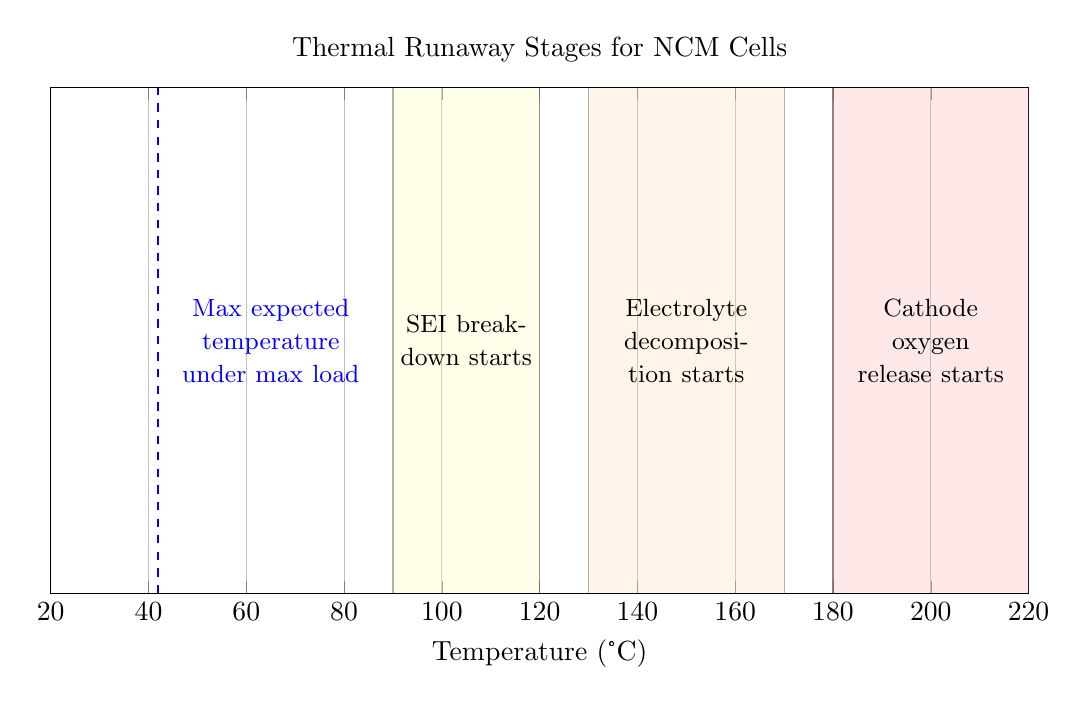
\begin{tikzpicture}
\begin{axis}[
    width=14cm, height=8cm,
    xlabel={Temperature (°C)},
    ylabel={},
    ytick=\empty,
    ymajorgrids=false,
    yminorgrids=false,
    grid=both,
    ymin=0, ymax=100,
    xmin=20, xmax=220,
    title={Thermal Runaway Stages for NCM Cells},
]

% SEI breakdown: 90-120°C
\draw[fill=yellow!30, opacity=0.3] (axis cs:90,0) rectangle (axis cs:120,100);
\node[align=center, text width=2cm] at (axis cs:105,50) {\small SEI breakdown starts};

% Electrolyte decomposition: 130-170°C
\draw[fill=orange!30, opacity=0.3] (axis cs:130,0) rectangle (axis cs:170,100);
\node[align=center, text width=2.5cm] at (axis cs:150,50) {\small Electrolyte decomposition starts};

% Cathode oxygen release: 180-220°C
\draw[fill=red!30, opacity=0.3] (axis cs:180,0) rectangle (axis cs:220,100);
\node[align=center, text width=2cm] at (axis cs:200,50) {\small Cathode oxygen release starts};

% Max operating temperature line (vertical)
\draw[blue, dashed, thick] (axis cs:42,0) -- (axis cs:42,100);
\node[blue, align=center, text width=2.5cm] at (axis cs:65,50) {\small Max expected temperature under max load};

\end{axis}
\end{tikzpicture}
\caption{Thermal runaway stages for NCM cells. Vertical blue dashed line shows estimated maximum cell temperature under maximum operation at ambient 40°C (42°C), well below the onset of SEI breakdown.}
\label{fig:thermal_safe}
\end{figure}

As shown in Figure~\ref{fig:thermal_safe}, even the highest credible thermal condition, corresponding to full-power discharge during a heatwave, remains far to the left of the first exothermic reaction zone. This separation demonstrates that the pack design operates well within thermally stable bounds under all foreseeable operating environments.

\section{Thermal Management and Environmental Control}

While active liquid or forced-air cooling is not necessary at the modest current densities used in this system, thermal management remains a central element of the overall safety architecture. The battery modules are installed within an open, ventilated enclosure that allows convective heat exchange with the surrounding air. The use of thermally conductive, flame-retardant interconnect materials further assists in spreading localised heat loads, ensuring no cell experiences abnormal temperature rise relative to its peers.

Environmental exposure is limited by physical shielding from direct solar radiation and precipitation, while the BMS enforces temperature-based operational constraints described in Section~\ref{sec:thermal-environment}. These limits prevent both lithium plating at low temperatures and accelerated SEI degradation at elevated ones—two of the principal precursors to cell instability.

The enclosure design also minimises the risk of heat accumulation through passive means. Airflow channels beneath and around the battery modules provide a continuous convection path, while thermal contact with metallic mounting plates helps distribute any localised heat generation. This ensures that even under sustained operation in warm ambient conditions, internal temperature gradients remain negligible.

A 100~A inline fuse provides a final passive failsafe, ensuring immediate isolation of the pack from external faults such as short circuits or controller failure. Together, these measures provide multi-layered protection: environmental control, passive thermal diffusion, conservative electrical limits (as detailed previously), real-time electronic protection, and a mechanical isolation barrier. Collectively, these controls ensure that even under single-fault conditions, cell temperatures remain well below the threshold of thermal instability.

\section{Electrical Protections and Fault Management}
\label{sec:electrical-protection}

The electrical protection architecture of the system has been designed to ensure immediate and deterministic responses to abnormal operating conditions, preventing both electrical overstress and secondary thermal effects.  
Protection functions are implemented at multiple levels: within the battery management system (BMS), through passive devices such as fuses, and by the motor controller’s firmware. This layered design provides redundancy and fail-safe isolation in the event of electrical faults.

The JK~BMS supervises each cell group individually, monitoring voltage, temperature, and current with millisecond-level resolution.  
If any cell exceeds its defined thresholds—overvoltage, undervoltage, overcurrent, or overtemperature—the BMS triggers a series of graded responses. These include immediate cessation of charging or discharging through solid-state contactor control, and, in extreme conditions, the activation of a physical relay to disconnect the entire pack from the vehicle’s electrical bus.  

An inline 100~A fuse is installed as a final passive safeguard. This component is rated to interrupt fault currents well in excess of the BMS cut-off limits and provides irreversible isolation in the event of catastrophic short circuits, such as wiring faults or controller failure.  
Fuse coordination analysis confirms that at 100~A continuous operation, the fuse remains thermally stable, while transient faults exceeding 300~A will result in disconnection within less than 100~ms.  

To prevent voltage imbalance that could otherwise lead to cell overcharge, the BMS includes active cell balancing circuitry. This system redistributes charge between parallel strings whenever voltage deviation exceeds 10~mV, maintaining pack uniformity and further reducing the risk of localised heating.  
The balancing current is deliberately limited to a modest level to ensure long-term stability and to avoid thermal stress on the cell interconnects.

Cables and busbars have been dimensioned according to AS/NZS 3008.1 and AS/NZS 5139:2019 for DC circuits at the expected continuous current. Conductor cross-sections were chosen such that the voltage drop remains below 2\%.  
All terminations use crimped and mechanically supported lugs to prevent loosening under vibration, and insulation is rated for at least 1.5~times the nominal pack voltage (i.e., 108~VDC continuous).  

\section{Physical and Fire Safety Design}

The battery pack enclosure is constructed from extruded aluminium, serving both as a passive heatsink and a robust containment vessel in the unlikely event of a thermal event. This design promotes uniform heat dissipation while maintaining mechanical protection against impact or vibration. A pressure relief vent is integrated to prevent enclosure rupture under gas expansion conditions, in accordance with AS IEC 62619 requirements.

The pack is mounted behind the operator’s compartment, separated by a fire-resistant barrier and accessible isolation switch. A Class D fire extinguisher is mounted within arm’s reach to address metal fires associated with lithium-based chemistries. All internal wiring employs double insulation, routed through grommeted bulkhead penetrations to minimise the risk of chafing and electrical faults. External conduits are rated for high temperature and abrasion resistance, contributing to a fail-safe electrical installation.

\section{Operational Controls and Training}

\subsection{Pre-Start Checklist}

Operators must complete a pre-start inspection before energising the traction system. The Battery Management System (BMS) automatically monitors and protects against out-of-range cell voltages, so manual voltage checking is not required. Instead, operators should confirm that the BMS status indicator shows no active faults or warnings.

A physical inspection must verify that the battery enclosure is cool to the touch (below approximately 40 °C) and free of any swelling, odour, or visible damage. All connectors should be confirmed secure, the primary fuse intact, and the fire extinguisher readily accessible and charged. This checklist reinforces operator awareness of physical and environmental safety conditions before operation.

\subsection{Charging Restrictions}

Battery charging must only occur in a well-ventilated area, on a non-combustible surface, and away from flammable materials such as fuels, solvents, or vegetation. The charging area must be supervised whenever the charger is energised. Operators must verify that charging cables and connectors are undamaged, clean, and properly latched before use. In the event of unusual noise, odour, or heat generation during charging, the charger must be immediately disconnected and the pack isolated for inspection. Charging should be avoided in direct sunlight or when ambient temperatures exceed 35 °C.

\subsection{Emergency Response}

In the event of a thermal anomaly or fire, the operator must immediately cease traction power and actuate the main isolation switch. A safe evacuation distance of at least 5~m should be maintained. The enclosure is designed to vent gases safely; therefore, direct water application is prohibited, as it may exacerbate thermal runaway. Once personnel are safe, the incident must be reported to incident control and the Office of the National Rail Safety Regulator (ONRSR) in accordance with safety management procedures.

\section{Testing and Commissioning Plan}

Before the traction system is approved for regular service, a structured commissioning process will be undertaken to validate all safety and performance functions under realistic operating conditions.

\begin{enumerate}
  \item Verify BMS cutoff voltages, charge current limits, and temperature protection by simulating charge and discharge events under supervision.
  \item Conduct an initial round-trip test over the full 3.3 km track, recording battery temperature, voltage, and current throughout the run. Confirm that peak cell temperature remains well below 60 °C and that no overcurrent or overtemperature faults are triggered.
  \item Validate fuse and MOSFET protection trip times through controlled short-duration overload tests.
  \item Confirm insulation resistance of the completed pack assembly exceeds \SI{1}{\mega\ohm} between conductors and the chassis.
  \item Document all measured data, thermal logs, and protection system responses, and file the results within the Safety Management System for review by the responsible engineer.
\end{enumerate}

\section{Post-Implementation Review Plan}

An initial review will occur after 25~operating hours or one month of service, whichever comes first. The inspection will focus on connection integrity, signs of thermal stress such as discolouration, and any evidence of corrosion or moisture ingress. Annual electrical testing will be conducted thereafter as part of the routine maintenance cycle of the vehicle.

\subsection{Electrical Work Scope and Authorisation}

All electrical work and modifications to the assist vehicle are performed in accordance with
the limits and definitions of \textbf{AS/NZS~3000:2018} and the Tasmanian Electrical Safety
Act 2022. The traction battery system operates at a nominal 72~V~DC, which falls within
the extra-low voltage (ELV) classification of the Wiring Rules (below 120~V ripple-free~DC).
Accordingly, work on the traction system may be carried out by technically competent
personnel trained in low-voltage battery systems, provided that the system remains isolated
from mains supply and incorporates the required protective measures.

All electrical assembly, modification, and maintenance tasks are undertaken by
appropriately trained personnel familiar with battery management, low-voltage design, and
traction applications.

% A licensed electrician, serving on the board of the Launceston \& North East Railway, provides formal inspection and verification of electrical integrity during commissioning and as part of the scheduled review process.

The mechanical integration of the traction motor, battery mounting, axles, and sprocket
assemblies has been completed by a qualified mechanic experienced in vehicle fabrication
and railway maintenance. All structural and drivetrain modifications have been carried out
to ensure mechanical robustness, alignment, and safety under expected operating loads.

The project has also been presented to the Australian Electric Vehicle Association (AEVA),
where it received positive feedback for its engineering approach and safety management.
This engagement demonstrates that the vehicle’s design and integration practices are
consistent with broader industry knowledge and accepted standards for low-voltage electric
mobility systems.

\section{Applicable Standards and References}

The design, installation, and operation of the modified assist vehicle have been carried out in accordance with recognised engineering and safety standards. \textbf{AS IEC 62619:2022}, which forms part of the original Hyundai Kona EV battery pack certification, has been followed and carries over to the modified vehicle, ensuring that the secondary lithium cells, battery assembly, and integration with the traction system meet internationally recognised requirements for thermal, electrical, and mechanical safety. Although \textbf{AS/NZS 5139:2019} applies to stationary energy storage systems, its safety principles have been applied as best-practice guidance in the installation and integration of the traction battery system to ensure appropriate protection, insulation, and control against fire, thermal runaway, and electrical faults. The wiring and electrical installation throughout the vehicle conforms to \textbf{AS/NZS 3000:2018} (Wiring Rules), ensuring proper conductor sizing, cable routing, and terminations. Operational procedures, pre-start checks, emergency response protocols, and personnel training have been conducted in line with \textbf{AS ISO 45001:2018}, addressing occupational health and safety management for all personnel operating or maintaining the modified vehicle.

\chapter{Validation \& Post-Implementation}

\section{Testing}

\printbibliography

\appendix

\chapter{Schematic}
\label{ch:schematic}

The following is an electronic schematic of the vehicle, along with a parts list. This document is printed in colour, laminated and stuck underneath the hood of the vehicle. Having documentation attached to the vehicle will make repairs safer, especially in the field, because details such as wiring and fusing are available.

\includepdf[pages=-,angle=90]{schematic.pdf}

\chapter{Safety Management System}
\label{ch:sms}

The following documents from the Safety Management System have been updated to reflect changes to the operation of the escort vehicle:

\begin{itemize}
    \item TRN/ASS-FRM-001 - Updated image of controls and answers
    \item OPS-PRO-005 - Removed fuel and oil check, added battery level, and added fire extinguisher check
    \item WI-FRM-004 - Removed fuel and oil check, added battery condition, removed transmission, and added chain tension
\end{itemize}

\includepdf[pages=-]{sms/TRN-ASS-FRM-001.pdf}

\includepdf[pages=-]{sms/OPS-PRO-005.pdf}

\includepdf[pages=-]{sms/WI-FRM-004.pdf}

\chapter{Simulation}
\label{ch:simulation}

The simulation software was written as an interactive webpage and is available online at \url{https://puffnfresh.github.io/rail-assist-vehicle-simulation/}. The source code for the project \href{https://github.com/puffnfresh/rail-assist-vehicle-simulation/blob/main/index.html}{is available on GitHub}. The simulation relies on a highly simplified physical model. The track is treated as a one-dimensional incline with a constant gradient, and resistance is reduced to rolling resistance plus the gravitational component of the combined mass. Dynamic effects such as acceleration transients, wheel slip, adhesion limits, and interactions between vehicles are omitted entirely. The calculations should be used as engineering estimates, rather than high-fidelity vehicle dynamics modelling.

\begin{figure}
  \includegraphics[width=\linewidth]{simulation-screenshot.png}
  \caption{Screenshot of the simulation webpage.}
%  \label{fig:bmsloom}
\end{figure}


\chapter{Photographic Evidence of Engineering Modifications}

\begin{figure}
  \includegraphics[width=\linewidth]{pics/battery-modules.jpg}
  \caption{Pallet of battery modules}
  \label{fig:batterymodules}
\end{figure}

\begin{figure}
  \includegraphics[width=\linewidth]{pics/20240730_125032.jpg}
  \caption{Briggs \& Stratton engine, before conversion.}
  \label{fig:before}
\end{figure}

\begin{figure}
  \includegraphics[width=\linewidth]{pics/motorplacement.jpg}
  \caption{Initial survey for motor placement}
  \label{fig:motorplacement}
\end{figure}

\begin{figure}
  \includegraphics[width=\linewidth]{pics/motorshaft.jpg}
  \caption{QS165 motor shaft}
  \label{fig:motorshaft}
\end{figure}

\begin{figure}
  \includegraphics[width=\linewidth]{pics/motormount1.jpg}
  \caption{Motor mount, showing bolting pattern}
  \label{fig:motormount1}
\end{figure}

\begin{figure}
  \includegraphics[width=\linewidth]{pics/motormount2.jpg}
  \caption{Motor mount, showing cable routing}
  \label{fig:motormount2}
\end{figure}

\begin{figure}
  \includegraphics[width=\linewidth]{pics/pulley1.jpg}
  \caption{Pulley which was determined to be too large}
  \label{fig:pulley1}
\end{figure}

\begin{figure}
  \includegraphics[width=\linewidth]{pics/pulley2.jpg}
  \caption{Pulley before machining to fit}
  \label{fig:pulley2}
\end{figure}

\begin{figure}
  \includegraphics[width=\linewidth]{pics/transmission.jpg}
  \caption{Transmission with a crookedly welded pulley}
  \label{fig:transmission}
\end{figure}

\begin{figure}
  \includegraphics[width=\linewidth]{pics/motorsprocket.jpg}
  \caption{Motor sprocket, 14 tooth, 428 profile}
  \label{fig:motorsprocket}
\end{figure}

\begin{figure}
  \includegraphics[width=\linewidth]{pics/axlesprocket.jpg}
  \caption{Axle sprocket, 40 tooth, 428 profile}
  \label{fig:axlesprocket}
\end{figure}

\begin{figure}
  \includegraphics[width=\linewidth]{pics/controllermount.jpg}
  \caption{Controller mount}
  \label{fig:controllermount}
\end{figure}

\begin{figure}
  \includegraphics[width=\linewidth]{pics/motormount3.jpg}
  \caption{Motor mounted to the rear chassis rail}
  \label{fig:motormount3}
\end{figure}

\begin{figure}
  \includegraphics[width=\linewidth]{pics/axlecoupler.jpg}
  \caption{Sprocket coupled to the axle}
  \label{fig:axlecoupler}
\end{figure}

\begin{figure}
  \includegraphics[width=\linewidth]{pics/chassismounted.jpg}
  \caption{Chassis, with motor and motor controller mounted}
  \label{fig:chassismounted}
\end{figure}

\begin{figure}
  \includegraphics[width=\linewidth]{pics/tensioner.jpg}
  \caption{Spring-loaded automatic chain tensioner}
  \label{fig:tensioner}
\end{figure}

\begin{figure}
  \includegraphics[width=12cm]{pics/batteryrack.jpg}
  \caption{Battery rack, on its side}
  \label{fig:batteryrack}
\end{figure}

\begin{figure}
  \includegraphics[width=\linewidth]{pics/testride.jpg}
  \caption{Initial test ride of vehicle, along the flat and straight at Turners Marsh station.}
  \label{fig:testride}
\end{figure}

\begin{figure}
  \includegraphics[width=12cm]{pics/fuse.jpg}
  \caption{Fuse, 100A, ANL-style}
  \label{fig:fuse}
\end{figure}

\begin{figure}
  \includegraphics[width=12cm]{pics/initialdash.jpg}
  \caption{Initial dashboard with emergency stop and beacon light}
  \label{fig:initialdash}
\end{figure}

\begin{figure}
  \includegraphics[width=12cm]{pics/charger.jpg}
  \caption{Adjustable voltage Li-ion charger}
  \label{fig:charger}
\end{figure}

\begin{figure}
  \includegraphics[width=\linewidth]{pics/bmsloom.jpg}
  \caption{BMS loom, wired to existing battery module sensor plugs}
  \label{fig:bmsloom}
\end{figure}

\begin{figure}
  \includegraphics[width=\linewidth]{pics/batteryandbms.png}
  \caption{Battery mounted in vehicle with BMS leads attached}
  \label{fig:batteryandbms}
\end{figure}

\begin{figure}
  \includegraphics[width=10cm]{pics/screenshotbms.png}
  \caption{Generic screenshot of BMS app}
  \label{fig:screenshotbms}
\end{figure}

\begin{figure}
  \includegraphics[width=10cm]{pics/screenshotfardriver.jpg}
  \caption{Generic screenshot of Fardriver app}
  \label{fig:screenshotfardriver}
\end{figure}

\begin{figure}
  \includegraphics[width=\linewidth]{pics/20250711_155137.jpg}
  \caption{Axle sprocket, 60 tooth, 428 profile}
  \label{fig:axlesprocket2}
\end{figure}

\begin{figure}
  \includegraphics[width=\linewidth]{pics/PXL_20251205_051644736.MP.jpg}
  \caption{Vehicle dashboard with forward/reverse selector, beacon indicator, emergency stop, speedometer, battery level indicator and horn button.}
  \label{fig:dashboard}
\end{figure}

\end{document}